\documentclass[spanish,]{article}
\usepackage{lmodern}
\usepackage{amssymb,amsmath}
\usepackage{ifxetex,ifluatex}
\usepackage{fixltx2e} % provides \textsubscript
\ifnum 0\ifxetex 1\fi\ifluatex 1\fi=0 % if pdftex
  \usepackage[T1]{fontenc}
  \usepackage[utf8]{inputenc}
\else % if luatex or xelatex
  \ifxetex
    \usepackage{mathspec}
  \else
    \usepackage{fontspec}
  \fi
  \defaultfontfeatures{Ligatures=TeX,Scale=MatchLowercase}
\fi
% use upquote if available, for straight quotes in verbatim environments
\IfFileExists{upquote.sty}{\usepackage{upquote}}{}
% use microtype if available
\IfFileExists{microtype.sty}{%
\usepackage{microtype}
\UseMicrotypeSet[protrusion]{basicmath} % disable protrusion for tt fonts
}{}
\usepackage[margin=1in]{geometry}
\usepackage{hyperref}
\hypersetup{unicode=true,
            pdftitle={CubOps: Manual de Usuario},
            pdfauthor={Julio Sergio Santana},
            pdfborder={0 0 0},
            breaklinks=true}
\urlstyle{same}  % don't use monospace font for urls
\ifnum 0\ifxetex 1\fi\ifluatex 1\fi=0 % if pdftex
  \usepackage[shorthands=off,main=spanish]{babel}
\else
  \usepackage{polyglossia}
  \setmainlanguage[]{spanish}
\fi
\usepackage{color}
\usepackage{fancyvrb}
\newcommand{\VerbBar}{|}
\newcommand{\VERB}{\Verb[commandchars=\\\{\}]}
\DefineVerbatimEnvironment{Highlighting}{Verbatim}{commandchars=\\\{\}}
% Add ',fontsize=\small' for more characters per line
\usepackage{framed}
\definecolor{shadecolor}{RGB}{248,248,248}
\newenvironment{Shaded}{\begin{snugshade}}{\end{snugshade}}
\newcommand{\KeywordTok}[1]{\textcolor[rgb]{0.13,0.29,0.53}{\textbf{#1}}}
\newcommand{\DataTypeTok}[1]{\textcolor[rgb]{0.13,0.29,0.53}{#1}}
\newcommand{\DecValTok}[1]{\textcolor[rgb]{0.00,0.00,0.81}{#1}}
\newcommand{\BaseNTok}[1]{\textcolor[rgb]{0.00,0.00,0.81}{#1}}
\newcommand{\FloatTok}[1]{\textcolor[rgb]{0.00,0.00,0.81}{#1}}
\newcommand{\ConstantTok}[1]{\textcolor[rgb]{0.00,0.00,0.00}{#1}}
\newcommand{\CharTok}[1]{\textcolor[rgb]{0.31,0.60,0.02}{#1}}
\newcommand{\SpecialCharTok}[1]{\textcolor[rgb]{0.00,0.00,0.00}{#1}}
\newcommand{\StringTok}[1]{\textcolor[rgb]{0.31,0.60,0.02}{#1}}
\newcommand{\VerbatimStringTok}[1]{\textcolor[rgb]{0.31,0.60,0.02}{#1}}
\newcommand{\SpecialStringTok}[1]{\textcolor[rgb]{0.31,0.60,0.02}{#1}}
\newcommand{\ImportTok}[1]{#1}
\newcommand{\CommentTok}[1]{\textcolor[rgb]{0.56,0.35,0.01}{\textit{#1}}}
\newcommand{\DocumentationTok}[1]{\textcolor[rgb]{0.56,0.35,0.01}{\textbf{\textit{#1}}}}
\newcommand{\AnnotationTok}[1]{\textcolor[rgb]{0.56,0.35,0.01}{\textbf{\textit{#1}}}}
\newcommand{\CommentVarTok}[1]{\textcolor[rgb]{0.56,0.35,0.01}{\textbf{\textit{#1}}}}
\newcommand{\OtherTok}[1]{\textcolor[rgb]{0.56,0.35,0.01}{#1}}
\newcommand{\FunctionTok}[1]{\textcolor[rgb]{0.00,0.00,0.00}{#1}}
\newcommand{\VariableTok}[1]{\textcolor[rgb]{0.00,0.00,0.00}{#1}}
\newcommand{\ControlFlowTok}[1]{\textcolor[rgb]{0.13,0.29,0.53}{\textbf{#1}}}
\newcommand{\OperatorTok}[1]{\textcolor[rgb]{0.81,0.36,0.00}{\textbf{#1}}}
\newcommand{\BuiltInTok}[1]{#1}
\newcommand{\ExtensionTok}[1]{#1}
\newcommand{\PreprocessorTok}[1]{\textcolor[rgb]{0.56,0.35,0.01}{\textit{#1}}}
\newcommand{\AttributeTok}[1]{\textcolor[rgb]{0.77,0.63,0.00}{#1}}
\newcommand{\RegionMarkerTok}[1]{#1}
\newcommand{\InformationTok}[1]{\textcolor[rgb]{0.56,0.35,0.01}{\textbf{\textit{#1}}}}
\newcommand{\WarningTok}[1]{\textcolor[rgb]{0.56,0.35,0.01}{\textbf{\textit{#1}}}}
\newcommand{\AlertTok}[1]{\textcolor[rgb]{0.94,0.16,0.16}{#1}}
\newcommand{\ErrorTok}[1]{\textcolor[rgb]{0.64,0.00,0.00}{\textbf{#1}}}
\newcommand{\NormalTok}[1]{#1}
\usepackage{graphicx,grffile}
\makeatletter
\def\maxwidth{\ifdim\Gin@nat@width>\linewidth\linewidth\else\Gin@nat@width\fi}
\def\maxheight{\ifdim\Gin@nat@height>\textheight\textheight\else\Gin@nat@height\fi}
\makeatother
% Scale images if necessary, so that they will not overflow the page
% margins by default, and it is still possible to overwrite the defaults
% using explicit options in \includegraphics[width, height, ...]{}
\setkeys{Gin}{width=\maxwidth,height=\maxheight,keepaspectratio}
\IfFileExists{parskip.sty}{%
\usepackage{parskip}
}{% else
\setlength{\parindent}{0pt}
\setlength{\parskip}{6pt plus 2pt minus 1pt}
}
\setlength{\emergencystretch}{3em}  % prevent overfull lines
\providecommand{\tightlist}{%
  \setlength{\itemsep}{0pt}\setlength{\parskip}{0pt}}
\setcounter{secnumdepth}{5}
% Redefines (sub)paragraphs to behave more like sections
\ifx\paragraph\undefined\else
\let\oldparagraph\paragraph
\renewcommand{\paragraph}[1]{\oldparagraph{#1}\mbox{}}
\fi
\ifx\subparagraph\undefined\else
\let\oldsubparagraph\subparagraph
\renewcommand{\subparagraph}[1]{\oldsubparagraph{#1}\mbox{}}
\fi

%%% Use protect on footnotes to avoid problems with footnotes in titles
\let\rmarkdownfootnote\footnote%
\def\footnote{\protect\rmarkdownfootnote}

%%% Change title format to be more compact
\usepackage{titling}

% Create subtitle command for use in maketitle
\newcommand{\subtitle}[1]{
  \posttitle{
    \begin{center}\large#1\end{center}
    }
}

\setlength{\droptitle}{-2em}
  \title{CubOps: Manual de Usuario}
  \pretitle{\vspace{\droptitle}\centering\huge}
  \posttitle{\par}
  \author{Julio Sergio Santana}
  \preauthor{\centering\large\emph}
  \postauthor{\par}
  \predate{\centering\large\emph}
  \postdate{\par}
  \date{19 de enero de 2018}


\begin{document}
\maketitle

{
\setcounter{tocdepth}{2}
\tableofcontents
}
\section{Introducción}\label{introduccion}

\textbf{CubOps} es una aplicación Web que le permitirá operar sobre un
conjunto de puntos, típicamente estaciones meteorológicas, cada uno de
los cuales contiene información temporal de un número finito de
variables, como pueden ser, precipitación, temperaturas mínimas y
máximas.

En general, el sistema trabaja con puntos a los que se le ha asociado un
número de variables cualquiera, que dependen de una fecha secuencial en
días.

Para el análisis y la aplicación de operaciones o producción de algunos
gráficos, el sistema permite generar una tabla completa para una
variable seleccionada, cada una de cuyas columnas corresponde a cada uno
de los puntos o estaciones de la base de datos. Posteriormente, se
pueden aplicar operaciones estadísticas (media, rango, mediana,
\emph{quantile}, etc.), a los datos de la columna, o a una selección de
esta de acuerdo con las fechas establecidas. El sistema también permite
la producción de varios tipos de gráficos simples para las columnas de
las tablas resultantes, a saber: histogramas, \emph{boxplots}, o series
de tiempo.

En cualquier momento, el usuario puede descargar las tablas resultantes
de sus operaciones en un formato estándar (csv), que podrá ser leído
fácilmente por hojas de cálculo, tales como \emph{LibreOffice Calc}, o
\emph{Excel}, o por otros sistemas o programas para desarrollar procesos
adicionales con la información.

\subsection{Bases de datos de ejemplo}\label{bases-de-datos-de-ejemplo}

Para que el usuario pueda experimentar con el sistema se proveen las
siguientes bases de datos para descargase en un equipo local:

\begin{enumerate}
\def\labelenumi{\arabic{enumi}.}
\tightlist
\item
  \href{http://172.16.19.27:3000/databases/UsumacintaDatos.zip}{Datos de
  más de 60 estaciones en la cuenca del río Usumacinta.}
\item
  \href{http://172.16.19.27:3000/databases/ConchosDatos.zip}{Datos de 14
  estaciones en la cuenca del río Conchos.}
\item
  \href{http://172.16.19.27:3000/databases/Estaciones.csv}{Información
  geográfica de ubicación las estaciones registradas en CLICOM.}
\end{enumerate}

Estos datos pueden utilizarse a partir de las acciones que se describen
a partir de la sección 3.5 (CubOps: colección de los datos).

\section{Aspecto general de CubOps}\label{aspecto-general-de-cubops}

Para ejecutar el sistema basta con introducir la siguiente URL en alguno
de los \emph{browsers} comunes de la Web, tales como Chrome o Firefox:

\url{http://172.16.19.27:3838/CubOps}

El sistema desplegará una interfaz al usuario, en la cual podrá
introducir sus peticiones y recibir sus respuestas. La Fig. 1 Muestra la
apariencia general del sistema una vez que se han desarrollado varias
operaciones. Al inicio de la sesión, sólo se muestra el menú etiquetado
como \textbf{Acción}, en el área \textbf{A} de la Fig. 1, y las áreas
\textbf{B} y \textbf{C} se muestran vacías, aunque, al pulsar en la
pestaña etiquetada como \textbf{Manual}, en el área \textbf{B}, se
desplegará el presente documento.

\begin{figure}
\centering
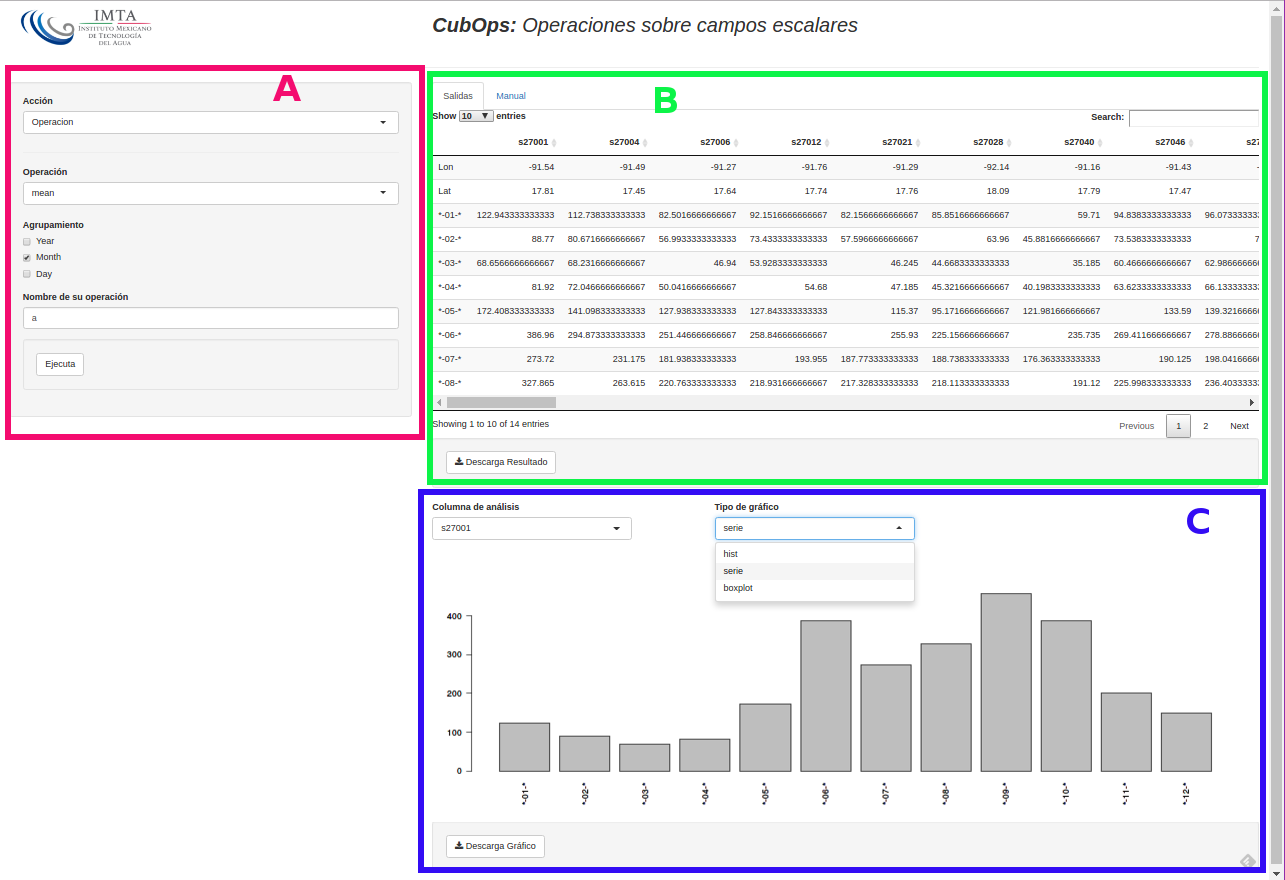
\includegraphics{CubOpsGral.png}
\caption{Apariencia general de CubOps}
\end{figure}

En esa figura se destacan la tres áreas principales del sistema, a
saber:

\begin{enumerate}
\def\labelenumi{\arabic{enumi}.}
\tightlist
\item
  \textbf{A}. \textbf{Panel de acciones}. Aquí el usuario define
  diversas acciones que van desde la captura de sus datos, hasta la
  operación sobre algún subconjunto de ellos para definir alguna
  estadística.
\item
  \textbf{B}. \textbf{Panel de resultados tabulares}. Los resultados
  tabulares de las operaciones se muestran en este espacio.
\item
  \textbf{C}. \textbf{Panel de operaciones y resultados gráficos}. Aquí
  el usuario puede definir diversos tipos de gráfico para alguna de las
  columnas del resultado tabular.
\end{enumerate}

\section{Los datos y su recolección}\label{los-datos-y-su-recoleccion}

Generalmente, los datos de cada estación estarán dados como una tabla en
la que se proporciona una fecha en cada renglón y con una columna para
cada una de las variables que se han registrado para la estación a lo
largo del tiempo. En seguida se muestran los diez primeros renglones de
una estación con tres variables: Prec (precipitación), Tmax (temperatura
máxima) y Tmin (temperatura mínima).

\begin{verbatim}
##    Year Month Day Prec Tmax Tmin
## 1  1951     1   1  0.0 31.3 17.6
## 2  1951     1   2  0.0 32.1 18.7
## 3  1951     1   3  0.0 32.1 18.3
## 4  1951     1   4  3.5 30.7 20.3
## 5  1951     1   5  0.0 30.7 19.7
## 6  1951     1   6  0.0 30.9 18.4
## 7  1951     1   7  0.0 30.8 17.9
## 8  1951     1   8  0.0 21.8 18.3
## 9  1951     1   9 20.0 23.6 14.3
## 10 1951     1  10  0.0 27.6 14.4
\end{verbatim}

De esta forma los datos de cada estación se pueden mantener en un
archivo de hoja de cálculo, como LibreOffice Calc o Excel. Para su
manejo en el presente sistema, dichos archivos deberán exportarse al
formato estándar CSV ( \emph{comma separated value} ), aunque ellos
podrán estar dispersos en una estructura de directorios o carpetas.

Los archivos CSV pudieran no traer el encabezado que identifica a cada
una de las columnas, pero en ese caso el sistema entenderá que, aparte
de la fecha que se debe dar en las primeras tres columnas, las columnas
restantes serán sólo tres que corresponderán a las variables pp
(precipitación), tmax (temperatura máxima) y tmin (temperatura mínima),
en ese orden.

\subsection{Los archivos y sus
nombres}\label{los-archivos-y-sus-nombres}

Para poder manejar dentro del sistema un conjunto de archivos de tablas
como las descritas en la sección 3, éstas se pueden encontrar dispersas
dentro de una estructura de directorios/subdirectorios (carpetas), del
sistema operativo, tal como se muestra en la Fig. 2. Sin embargo, para
que el sistema pueda reconocer los archivos en cuestión, ellos deben ser
nombrados de acuerdo con una estructura sintáctica particular que se
describe a continuación:

\begin{enumerate}
\def\labelenumi{\arabic{enumi}.}
\tightlist
\item
  El primer caracter del nombre debe ser una letra ``s'', minúscula.
\item
  En seguida, una secuencia de caracteres alfanuméricos que representan
  el \emph{identificador} de la estación correspondiente al archivo.
\item
  Después una letra ``H'', mayúscula y la secuencia de caracteres
  ``.csv'', que identifican el tipo de archivo.
\end{enumerate}

Por ejemplo, el archivo de nombre ``s3394H.csv'' contendría la tabla de
información de la estación 3394 en formato CSV. A estos archivos se les
denominará \emph{archivos de estaciones}.

\subsection{Los archivos y su
estructura}\label{los-archivos-y-su-estructura}

Externamente, como se mustra en la Fig. 2, los archivos de estaciones
podrán estar dispersos en una estructura de directorios. Internamente,
la condición es que la estructura de las tablas sea la misma para todos
los archivos, esto es, todos deben tener el mismo número de columnas,
con las tres primeras para la fecha en orden: año, mes y día, y las
restantes para las variables que se registren en las estaciones, en el
mismo orden para todas las tablas. Si las tablas llevan o no encabezado,
esto debe ser igual para todas ellas.

\begin{figure}
\centering
\includegraphics{DirStruct.png}
\caption{Ejemplo de estructura de directorios con archivos CSV}
\end{figure}

\subsection{Empaquetado de los
archivos}\label{empaquetado-de-los-archivos}

Para que el sistema pueda digerir la información correspondiente a un
conjunto de estaciones como la que se ha ilustrado en las secciones
anteriores y que se muestra gráficamente en la Fig. 2, es necesario
empaquetarlo en un solo archivo de tipo ZIP.

En un sistema operativo Linux o Unix, el comando para efectuar esa
operación es:

\begin{Shaded}
\begin{Highlighting}[]
\FunctionTok{zip}\NormalTok{ -r arch.zip path/de/inicio}
\end{Highlighting}
\end{Shaded}

Al final de la operación toda la estructura de archivos se tendría en el
paquete de nombre ``arch.zip'', en el caso del ejemplo.

\subsection{Información geográfica de
estaciones}\label{informacion-geografica-de-estaciones}

Aparte de la información de diversas variables de las estaciones, que se
empaca en un archivo de tipo ZIP, como se ha mostrado en las secciones
anteriores, es necesario proveer también de una tabla que registre las
coordenadas geográficas en formato CSV. Un ejemplo de la estructura de
esta tabla se muestra a continuación:

\begin{verbatim}
##    Clave                  Nombre  Latitud  Longitud
## 1   1003          CALVILLO (SMN) 21.88333 -102.7189
## 2   1004            CA?ADA HONDA 22.00778 -102.1981
## 3   1005        PRESA EL NIAGARA 21.77889 -102.4414
## 4   1006           EL TULE (SMN) 22.08167 -102.0914
## 5   1007       JESUS MARIA (SMN) 21.96222 -102.3447
## 6   1008 PUERTO DE LA CONCEPCION 22.20250 -102.1344
## 7   1009          LA LABOR (SMN) 21.96222 -102.6947
## 8   1010               LA TINAJA 22.16528 -102.5558
## 9   1011                 MALPASO 21.85833 -102.6628
## 10  1012        PRESA MEDIA LUNA 21.79250 -102.8017
\end{verbatim}

La tabla debe contener por lo menos tres columnas, la correspondiente a
la ``Clave'' de la estación, y las correspondientes a la ``Longitud'' y
``Latitud'' de la estación, con esos nombres de columna. Además, la
tabla debe contener \emph{al menos} la información de las estaciones que
se consignan en el empaquetamiento de la sección 3.3.

\subsection{CubOps: colección de los
datos}\label{cubops-coleccion-de-los-datos}

Para que el sistema colecte toda la información de las estaciones se
debe seleccionar, en el menú de Acciones, la entrada ``\textbf{Colecta
Datos}'', como se muestra en la Fig. 3.

\begin{figure}
\centering
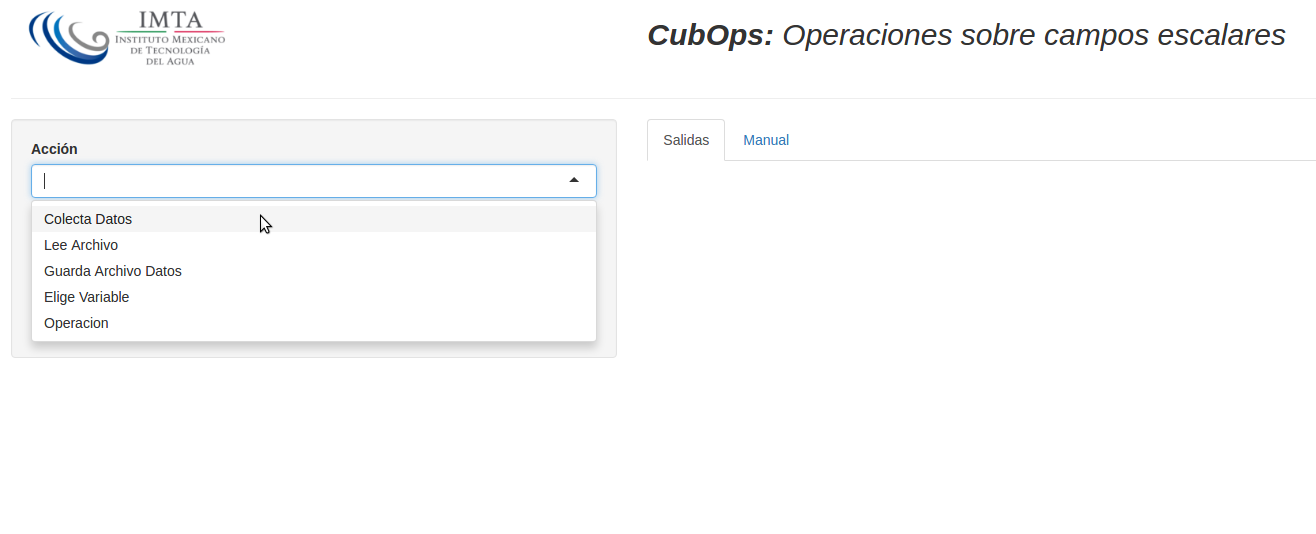
\includegraphics{ColeccionDatos1.png}
\caption{Colección de datos}
\end{figure}

Una vez seleccionada esta acción el sistema provee sendos botones para
la \emph{subida} de los dos archivos de interés, descritos en las
secciones 3.3 y 3.4; esto es, el paquete de archivos ZIP con la
información de las variables en las estaciones y el archivo CSV con la
información geográfica de las estaciones. El despliegue de estos botones
se muestra en la Fig. 4, a continuación.

\begin{figure}
\centering
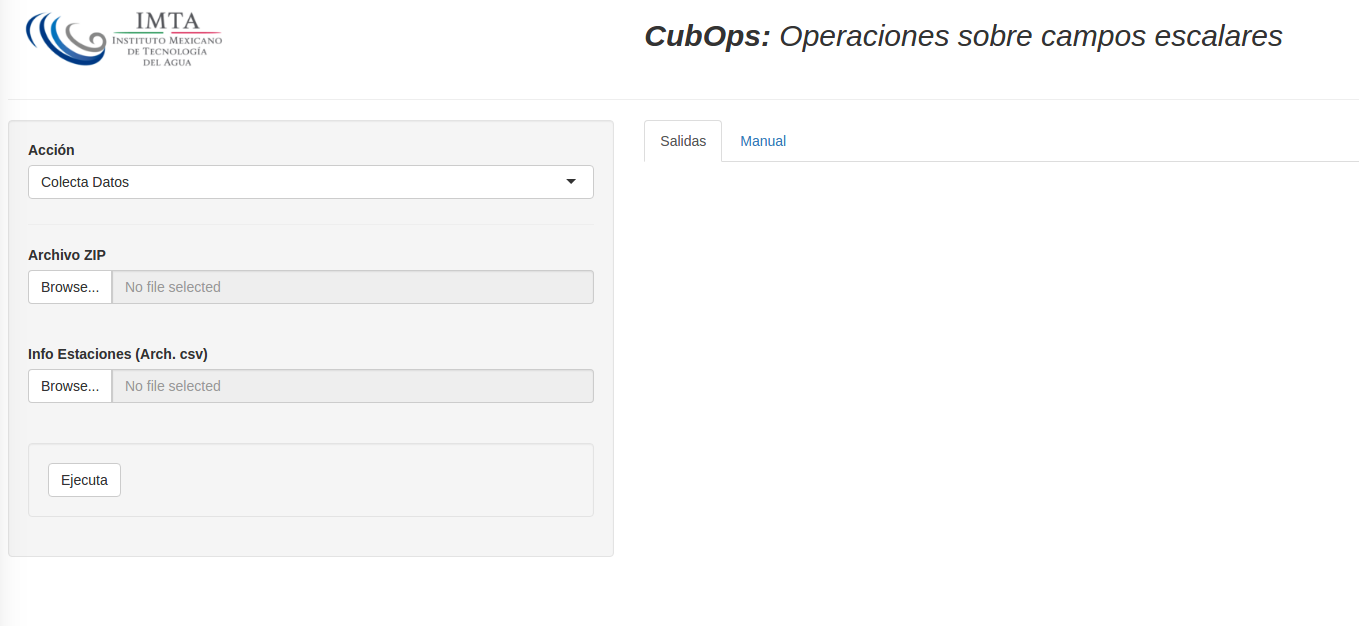
\includegraphics{ColeccionDatos2.png}
\caption{Botones para la \emph{subida} de archivos de datos}
\end{figure}

Ya que se han subido o cargado estos datos, lo cual se muestra en las
barras de progreso de la carga en la Fig. 5, se debe oprimir el botón
``\textbf{Ejecuta}'', en la parte inferior del panel de Acciones, para
proceder al armado completo de la estructura de información que utiliza
internamente el sistema. En la Fig. 5, se muestra el resultado, donde,
en el panel de resultados tabulares, se muestra un texto que da alguna
pista del armado de dicha estructura.

\begin{figure}
\centering
\includegraphics{ColeccionDatos4.png}
\caption{Armado de la estructura de información}
\end{figure}

\subsection{Descarga y recarga de la estructura de
información}\label{descarga-y-recarga-de-la-estructura-de-informacion}

Una vez construída la estructura de información, como se ha mostrado en
las secciones anteriores, ésta se puede descargar de manera local para
reutilizarse posteriormente por el sistema, sin necesidad de
reconstruírla a partir de un archivo de tipo ZIP. La descarga se hace
seleccionando la entrada ``\textbf{Guardar Archivo Datos}'', en el menú
de acciones (ver Fig. 3). La estructura de información queda guardada en
un archivo de tipo RDS, que es un archivo binario del lenguaje de
programación R.

La recarga de la estructura de información, se hace seleccionando la
entrada ``\textbf{Lee Archivo}'', en el menú de Acciones (ver Fig. 3).
Una vez leído algun archivo de este tipo (RDS), el resultado sería
semejante al de la construcción de la estructura que se muestra en la
Fig. 5.

\section{Selección de variables}\label{seleccion-de-variables}

El sistema maneja una estructura de información que se ha construído
como se ha señalado en las secciones anteriores. La Fig. 6 muestra de
manera gráfica la apariencia de dicha estructura.

\begin{figure}
\centering
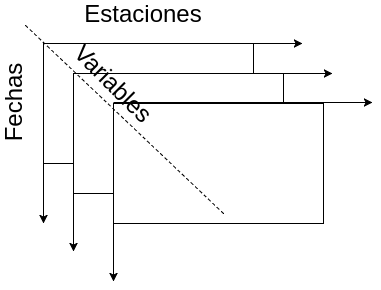
\includegraphics{Cubote.png}
\caption{La estructura de la información}
\end{figure}

La estructura puede ser concebida como \emph{un número determinado de
tablas}, tantas como variables haya registradas, cuyos renglones serían
las fechas y cuyas columnas corresponderían con cada una de las
estaciones (ver Fig. 6). El presente sistema permite operar sobre cada
una de las tablas de la estructura; esto es, con cada una de las
variables registradas. De modo que el primer paso, antes de cualquier
operación, es la selección de una tabla o variable para trabajar con
ella.

Para proceder a la selección de la variable, se debe entrar al menú de
Acciones y seleccionar de ahí la entrada ``\textbf{Elige Variable}''
(ver Fig. 3). Esta acción abre un menú, ``\textbf{Variable a revisar}'',
con el conjunto de variables que se pueden revisar, como se muestra en
la Fig. 7.

\begin{figure}
\centering
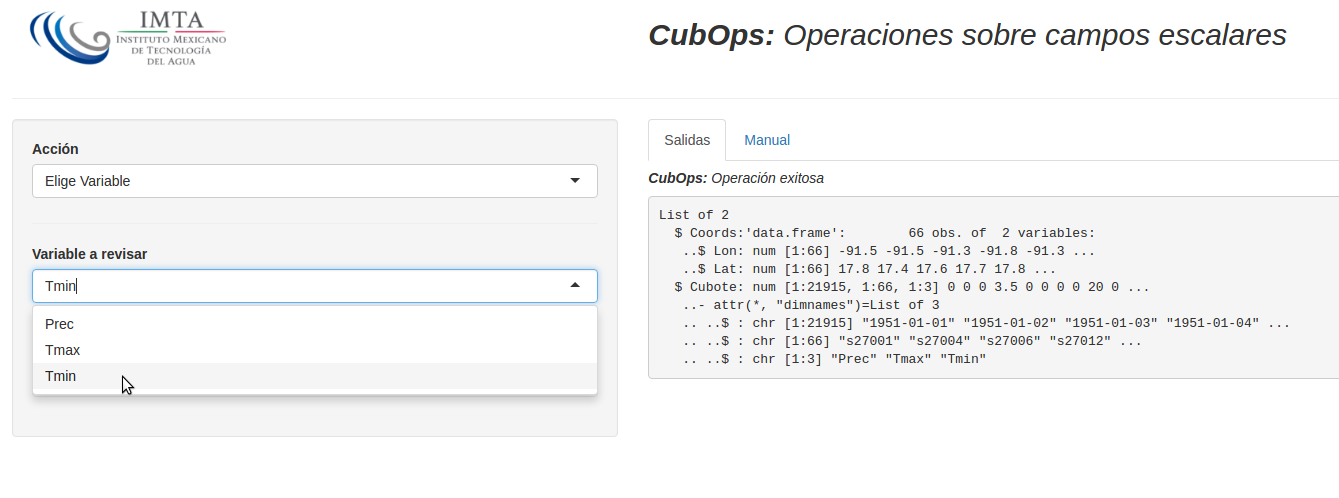
\includegraphics{SelVar.png}
\caption{Conjunto de variables que pueden ser revisadas}
\end{figure}

Una vez que se elige la variable deseada, y luego de que se oprime el
botón ``\textbf{Ejecuta}'', en el panel de resultados tabulares, aparece
la tabla correspondiente a la variable, con los dos primeros renglones
mostrando las coordenadas geográficas de las estaciones. La tabla se
puede navegar por páginas. Este resultado se muestra abajo en la Fig. 8.

\begin{figure}
\centering
\includegraphics{SelVar1.png}
\caption{Tabla correspondiente a una variable}
\end{figure}

La tabla resultante, se puede descargar a su equipo local, en el formato
estándar CSV, oprimiendo el botón ``\textbf{Descarga Resultado}'', que
aparece en la parte inferior del panel de resultados tabulares (Ver Fig.
8).

\subsection{Selección de variables y
operaciones}\label{seleccion-de-variables-y-operaciones}

En la sección siguiente se empieza a tratar el asunto de la aplicación
de operaciones sobre los datos contenidos en la tabla o variable
seleccionada. Dado que \textbf{las operaciones se aplican sobre la tabla
visible}, cada vez que se quiera aplicar una nueva operación sobre los
mismos datos, será necesario \emph{regresar} y elegir nuevamente la
misma variable para restablecer la tabla de origen. Esto, como se verá
más adelante en la sección 6.3, es porque hay resultados que se
obienenen de aplicar consecutivamente varias operaciones sobre las
tablas consecutivas resultantes, por ejemplo, en el caso de los
promedios de sumas acumulativas de precipitación.

\section{Operaciones estadísticas sobre columnas
completas}\label{operaciones-estadisticas-sobre-columnas-completas}

El sistema permite ejecutar alguna de las operaciones estadísticas
disponibles, sobre la series completas de datos de todas las columnas
exhibidas, que corresponden a las estaciones registradas. Como se verá
más adelante, algunas operaciones, como la media, la varianza, o la
mediana, reportarán un sólo resultado numérico para cada serie de datos,
mientras que otras, como el rango o los cuantiles, reportarán dos o más
resultados.

Para seleccionar una operación cualquiera, primeramente se toma del menú
de Acciones, la entrada ``\textbf{Operación}'', lo que abre un menú de
``\textbf{Operación}'' con todas las operaciones estadísticas
disponibles, tal como se muestra en la Fig. 9. Al momento, las
operaciones disponibles son: la media (mean), la mediana
(\textbf{median}), la varianza (\textbf{var}), la desviación estándar
(\textbf{sd}), la sumatoria (\textbf{sum}), el valor mínimo
(\textbf{min}), el valor máximo (\textbf{max}), el rango
(\textbf{range}), compuesto por los valores mínimo y máximo, y los
cuantiles (\textbf{quantile}).

\begin{figure}
\centering
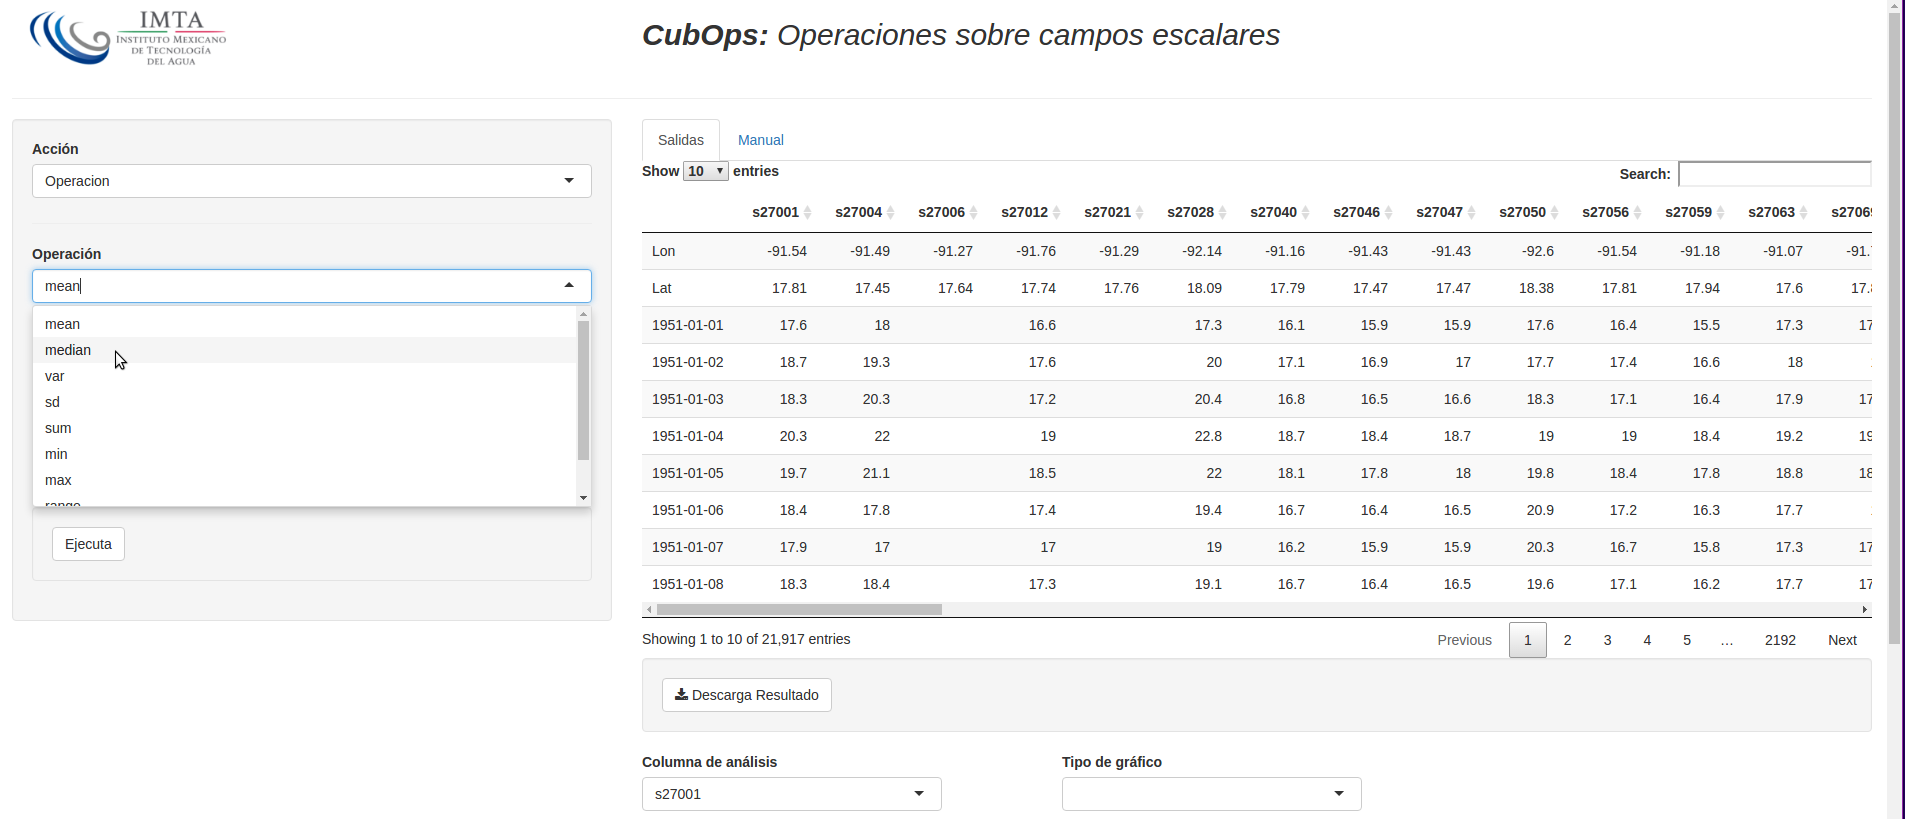
\includegraphics{SelOper.png}
\caption{Menú de operaciones}
\end{figure}

Nótese, en la Fig. 9, que en la tabla sobre la cuál se va a operar, hay
columnas sin datos, tales como las etiquetadas ``s27006'' y ``s27021''.

Ya que se ha elegido la operación, por ejemplo \emph{la mediana}, y se
le ha dado un nombre, en el campo textual provisto para ello, por
ejemplo ``mm'', se procede a ejecutar dicha operación, para todas las
columnas con datos al oprimir el botón ``\textbf{Ejecuta}'' que aparece
en la parte inferior del panel de acciones. Los resultados de la
operación se muestran en una tabla como la que se muestra en la Fig. 10,
donde la operación en cuestión arroja un único resultado para cada serie
de datos (columna).

\begin{figure}
\centering
\includegraphics{SelOper1.png}
\caption{Operación de \emph{un solo resultado} (mediana)}
\end{figure}

Nuevamente, la tabla resultante puede ser descargada en un equipo local,
en el formato estándar CSV, al oprimir el botón ``\textbf{Descarga
Resultado}''.

\subsection{Operaciones con más de un resultado:
cuantiles}\label{operaciones-con-mas-de-un-resultado-cuantiles}

Como se mencionó antes, hay operaciones estadísticas que arrojarán más
de un dato a la salida. Tal es el caso de los cuantiles. Si se elige
esta operación en el menú de ``\textbf{Operación}'', la interfaz del
sistema despliega un campo de texto etiquetado como
``\textbf{Probabilidades separadas por','}'', en el que se pueden
especificar las probabilidades de \emph{ruptura}, separadas por comas,
de los cuantiles para el cálculo. Por omisión, estas probabilidades son:
0, 0.25, 0.50, 0.75 y 1.0, lo que corresponde a los así denominados
\emph{cuartiles} de cada serie. El resultado, que se muestra en la Fig.
11, estaría dado, en ese caso, por 5 renglones, nombrados como: qq.0\%,
qq.25\%, qq.50\%, qq.75\% y qq.100\%. El prefijo ``qq'' en todos los
nombres de los renglones de la tabla, se ha tomado del campo de texto
``\textbf{Nombre de su operación}'', que es un nombre arbitrario que
provee el usuario del sistema.

\begin{figure}
\centering
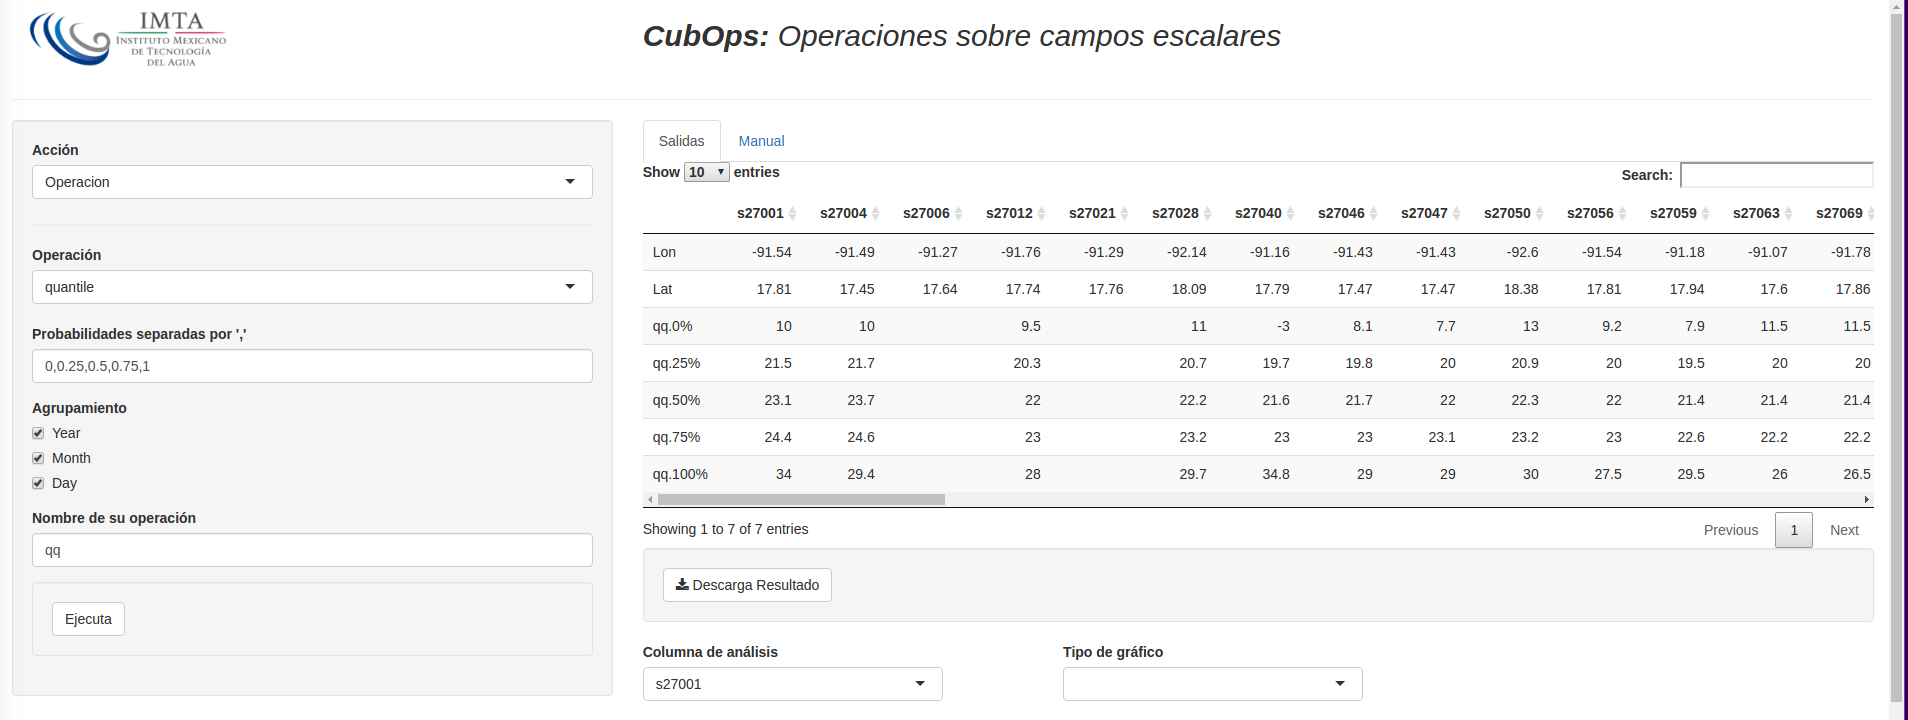
\includegraphics{SelOper2.png}
\caption{Cuartiles para cada una de las columnas}
\end{figure}

La interpretación de la información en esa tabla es más o menos
sencilla. Por ejmplo, para la primera columna, etiquetada como
``s27001'', la serie de datos de temperatura mínima, que fue la variable
elegida, tienen un valor mínimo y máximo de 10° y 34°, que en la columna
se muestran como los renglones qq.0\% y qq.100\%, respectivamente, lo
que se interpreta como 0\% de los datos están tienen un valor menor que
10° y 100\% de los datos, esto es, todos, tienen un valor menor o igual
que 34°. En este caso, la mediana de los datos es 23.1°, lo que
significa que el 50\% de los datos es menor o igual a este valor
(qq.50\%).

Cambiar las probabilidades en el campo de texto, permite desarrollar el
calculo de otro tipo de cuantiles. Por ejemplo, si se quisieran calcular
los terciles, se podría establecer la siguiente serie de probabilidades:
0, 0.3333, 0.6667, y 1.0. El resultado de esta operación se muestra en
la Fig. 12.

\begin{figure}
\centering
\includegraphics{SelOper3.png}
\caption{Terciles para cada una de las columnas}
\end{figure}

Nuevamente, en cualquiera de estos casos, la tabla resultante, por
ejemplo, con cuartiles o terciles, puede ser descargada en un equipo
local, en el formato estándar CSV, al oprimir el botón
``\textbf{Descarga Resultado}''.

Nótese además, que las columnas que no tenían información originalmente,
tampoco reportan resultados en ninguno de los dos casos ejemplificados.

\section{Estratificaciones de datos y operaciones sobre
ellas}\label{estratificaciones-de-datos-y-operaciones-sobre-ellas}

Al aplicar las distintas operaciones estadísticas, las fechas, que obran
como nombre de los renglones de la tabla, se pueden usar para ejecutar
distintas \emph{estratificaciones} de los datos. Se puede definir como
un \emph{\textbf{estrato}} de una \emph{estratificación}, al conjunto de
renglones que comparten alguna porción de la fecha, por ejemplo, el año
y el mes; esto es, por ejemplo, los 31 renglones del mes de marzo de
1961, constituirían un estrato para ese caso. La
\emph{\textbf{estratificación}} sería entonces el conjunto de todos los
estratos que la componen.

\subsection{Definición de una estratificación en
CubOps}\label{definicion-de-una-estratificacion-en-cubops}

Después de haber seleccionado alguna variable, y al momento de elegir
alguna operación, se puede definir también alguna estratificación a
partir de las fechas. Esto se hace, mediante el agrupamiento en los
campos de fecha, como se muestra en la Fig. 13.

\begin{figure}
\centering
\includegraphics{Estratif.png}
\caption{Agrupamientos}
\end{figure}

En el caso de la Fig. 13, se ha elegido el año y el mes, mientras que el
día se ha descartado. Esto significa que los estratos se definirán a
partir del año y el mes solamente. Esto es, la operación que se elija,
la media en este caso, se ejecutará para los conjuntos de renglones que
tengan el mismo año y mes, o sea, se estarán obteniendo los promedios
mensuales de temperatura mínima a lo largo de todos los años en el
registro. Así, la Fig. 14, muestra el resultado de esta operación.
Nótese que en las fechas, el campo correspondiente al día se ha
reemplazado por un asterisco ``*''. Entonces, por ejemplo, el primer
dato de la columna etiquetada como ``s27001'', se encuentra en el
renglón ``1951-01-*''; ello indica que la media de temperaturas mínimas
durante el primer mes de año 1951 es de 16.887°, y así son también todas
las interpretaciones de todas las columnas y renglones de la tabla
resultante.

\begin{figure}
\centering
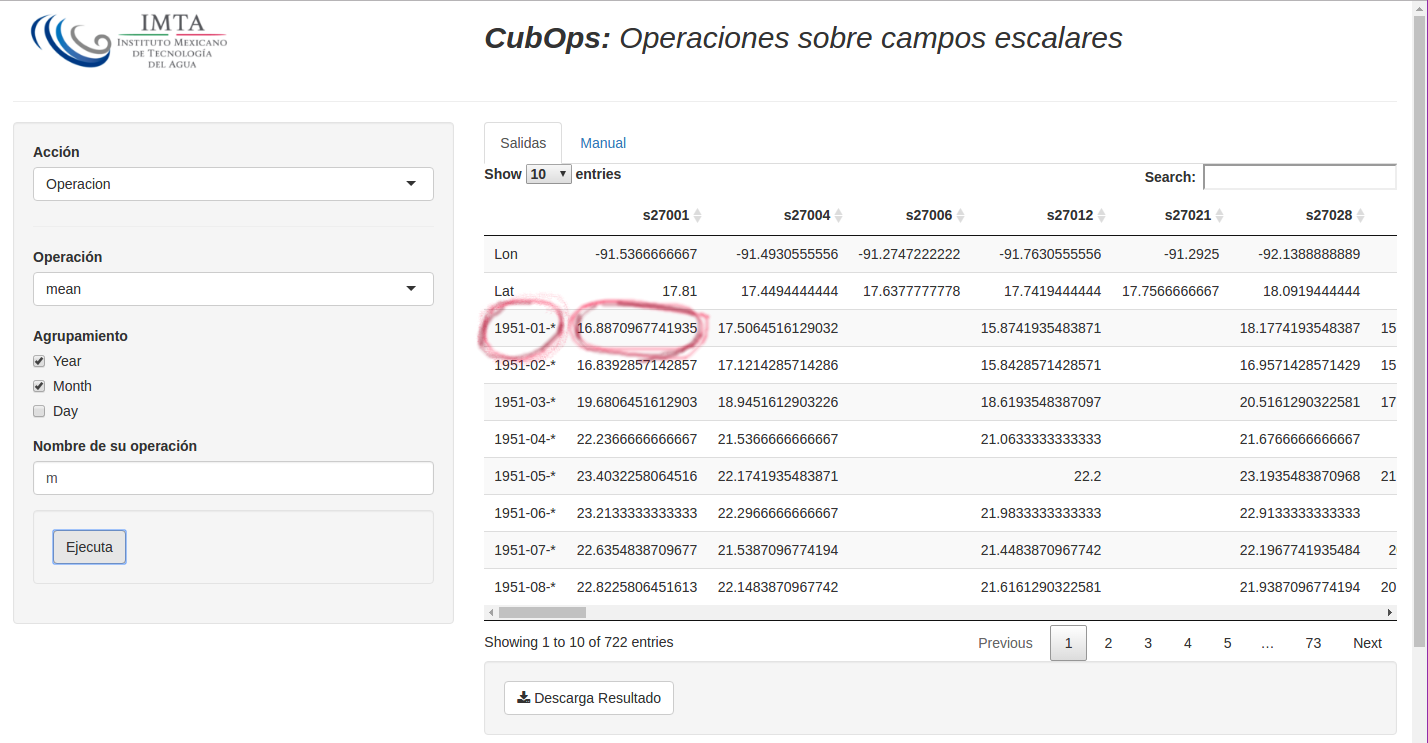
\includegraphics{OpEstratif.png}
\caption{Resultados de una operación estratificada}
\end{figure}

Nuevamente, esta tabla resultante, puede ser descargada en un equipo
local, en el formato estándar CSV, al oprimir el botón
``\textbf{Descarga Resultado}''.

\subsection{Estratificaciones y operaciones con resultados
múltiples}\label{estratificaciones-y-operaciones-con-resultados-multiples}

Cuando se ejecutan operaciones combinadas con estratificaciones de la
tabla, se puede ver en la Fig. 14, que la tabla resultante arroja un
renglón para cada estrato de los datos originales. Esto no representa
ningún problema si la operación arroja un único resultado, como es el
caso de la media, la mediana, o la desviación estándar, por ejemplo. En
este punto surge la pregunta: ¿cómo maneja CubOps el caso de operaciones
que arrojan más de un resultado?, ya que por cada estrato y estación se
tendrían resultados múltiples. La respuesta es que el sistema
\emph{\textbf{expande la columna correspondiente a una estación, a
tantas columnas como resultados arroje la operación en cuestión}}. La
Fig. 15 muestra, como ejemplo, el caso de la producción de
\emph{terciles}, por medio de la operación ``\textbf{quantile}'', para
una tabla original de temperaturas mínimas. Es de notarse aquí que los
nombres de las columnas están formados por el nombre de la estación
original, seguido del caracter ``:'', y luego un conjunto de caracteres
que permitirán identificar cada caso, que para el ejemplo de los
terciles son los porcentajes de probabilidad elegidos.

\begin{figure}
\centering
\includegraphics{EstratifMultpl.png}
\caption{Terciles para datos estratificados}
\end{figure}

\subsection{Aplicación recurrente de
operaciones}\label{aplicacion-recurrente-de-operaciones}

Hay ocasiones en que es necesario aplicar una nueva operación al
resultado de otra operación. Tal es el caso de los \textbf{promedios
mensuales de precipitaciones acumuladas durante el mes}. Con este
propósito, CubOps ha sido diseñado para aplicar cualquiera de las
operaciones disponibles sobre la tabla actualmente visible en el panel
de resultados tabulares.

Por ejemplo, para producir justamente los \textbf{promedios mensuales de
precipitaciones acumuladas durante el mes}, primeramente se selecciona
la variable precipitación de la estructura de información vigente, como
se muestra en la Fig. 16.

\begin{figure}
\centering
\includegraphics{Recurr0.png}
\caption{Selección de la variable precipitación}
\end{figure}

Ahora se procede a acumular las precipitaciones que ocurrieron cada mes,
para ello se selecciona la operación \textbf{sum} (sumatoria), y en el
\textbf{Agrupamiento} se elimina el campo correspondiente al día, con el
fin de producir estratos mensuales para todos los años, tal como se
muestra en la Fig. 17. Ahí, por ejemplo, en el renglón ``1951-03-*'' y
la columna ``s27004'', se encuntra el valor 133.6, lo que significa que
durante el mes de marzo del año 1951, se observó una precipitación
acumulada durante todo el mes de 133.6 mm en la estación 27004.

\begin{figure}
\centering
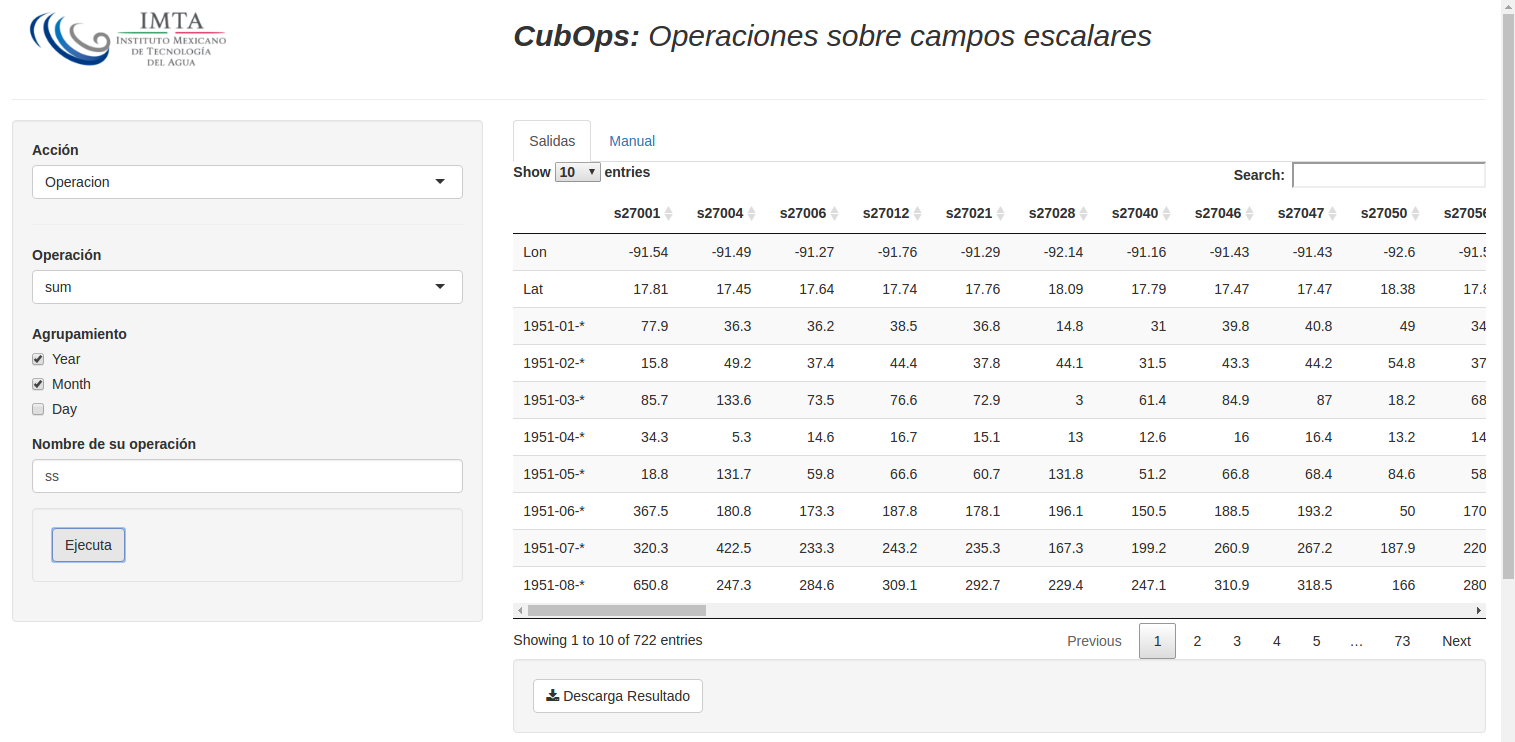
\includegraphics{Recurr1.png}
\caption{Acumulación de precipitaciones por mes}
\end{figure}

Finalmente, para producir los promedios mensuales de esos resultados
para toda la serie, se procede a elegir la operación \textbf{mean} y se
elimina ahora el campo correspondiente al año en el
\textbf{Agrupamiento}. Después de oprimir el botón \textbf{Ejecuta}, se
obtiene el resultado que se muestra en la Fig. 18. En el renglón
``*-09-*'' y columna ``s27021'', se observa un valor de 322.705, lo que
significa que el promedio de precipitaciones acumuladas mensuales en el
mes de septiembre, para la estación 27021, es de 322.705 mm.

\begin{figure}
\centering
\includegraphics{Recurr2.png}
\caption{Promedios de precipitaciones acumuladas mensuales}
\end{figure}

\section{Gráficas sencillas con
CubOps}\label{graficas-sencillas-con-cubops}

Como una cualidad adicional, \textbf{CubOps} permite generar algunos
tipos de gráficas sencillas, a saber: series, histogramas y
\emph{boxplots} (diagramas de cajas). Estas gráficas permiten tener una
mayor visión general de los resultados que se presentan en las tablas
del panel de resultados tabulares. A continuación se indica cómo
explotar esta característica del sistema.

\subsection{Gráficos de información completa de estaciones
(columnas)}\label{graficos-de-informacion-completa-de-estaciones-columnas}

Después de elegir alguna de las variables disponibles, como es el caso
que se ha presentado en la Fig. 8, se puede proceder a producir alguna
de las gráficas disponibles. Para ello es necesario primeramente,
seleccionar alguna de las columnas en la tabla y luego el tipo de
gráfico deseado. Por ejemplo, en la Fig. 19 se ha seleccionado la
columna ``s27040'' y se ha elegido la producción de un gráfico de tipo
``hist'' (histograma); después de esa selección el gráfico
correspondiente se muestra en la parte inferior, conocida como
\emph{panel de resultados gráficos}. El gráfico producido se puede
salvar en un archivo gráfico, si se oprime el botón etiquetado como
\textbf{Descarga Gráfico}.

\begin{figure}
\centering
\includegraphics{Graf1.png}
\caption{Producción de gráficos con \textbf{CubOps}}
\end{figure}

Para el caso particular de los histogramas, aparece además un control,
conocido como \emph{slider}, que permite incrementar o disminuir el
número de barras que se presentan en el histograma. Al desplazar de
botoncito, dinámicamente se incrementan o decrementan las barras que
aparecen, como se puede apreciar el la Fig. 20.

\begin{figure}
\centering
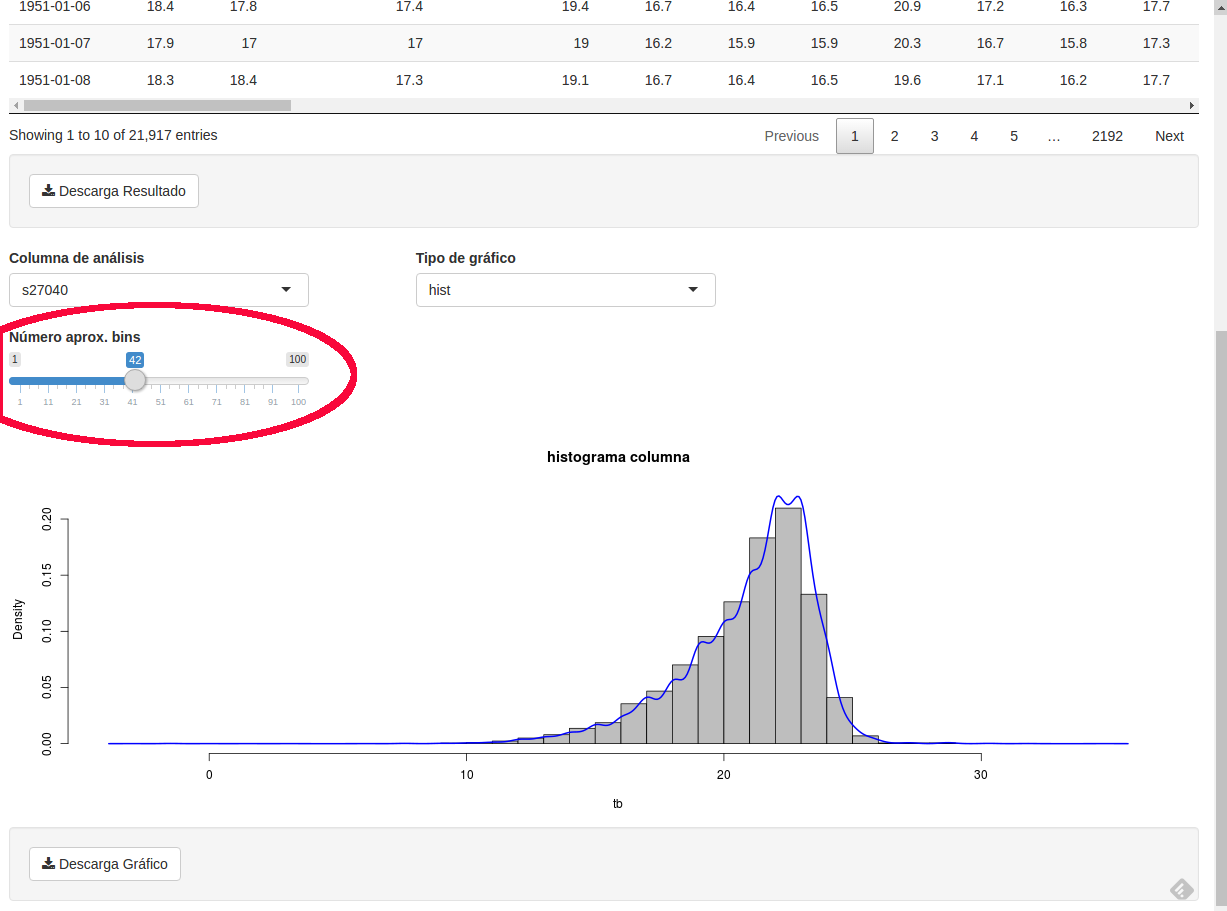
\includegraphics{Graf2.png}
\caption{Otros controles en las gráficas}
\end{figure}

\subsection{Algunos usos de los
gráficos}\label{algunos-usos-de-los-graficos}

Cuando ya se ejecutan operaciones en las estaciones o columnas, los
gráficos producidos pueden ser más interesantes. Por ejemplo, en la Fig.
21, se observa un gráfico de tipo ``serie'', que se ha producido después
de haber ejecutado la operación ``quantil'' sobre todos los datos de
temperatura mínima de la columna ``s27040''. Aquí, en el eje de las
abscisas se tienen los rangos de cuantil, y en las ordenadas, los
valores de las temperaturas.

\begin{figure}
\centering
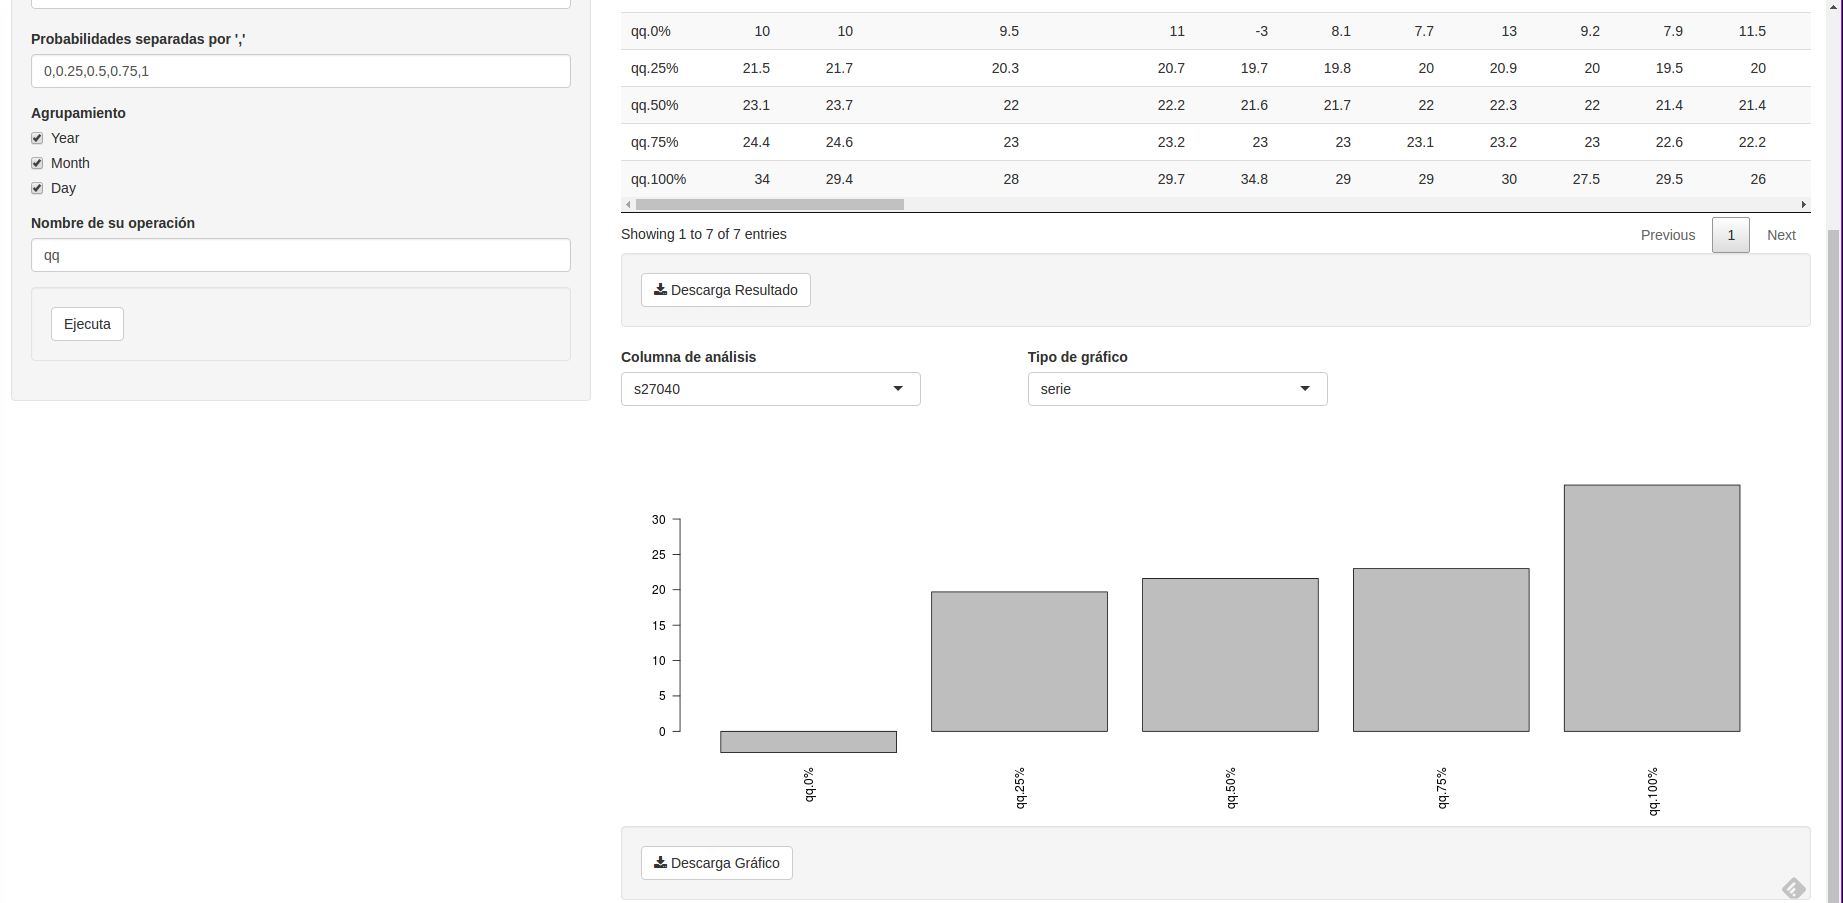
\includegraphics{Graf3.png}
\caption{Gráfica de los cuantiles}
\end{figure}

Otro interesante gráfico a considerar son los \emph{boxplots}, que dan
también una idea de la distribución de la información. La Fig. 22
muestra un gráfico de este tipo para las temperaturas mínimas de la
estación ``s27004''.

\begin{figure}
\centering
\includegraphics{Graf4.png}
\caption{Gráfica tipo \emph{boxplot}}
\end{figure}

Un caso interesante es la graficación de la climatología de las
precipitaciónes acumuladas mensuales, cuyo cálculo se ha presentado en
forma tabular en la Fig. 18. Para graficar esto, basta con seleccionar
alguna estación y el tipo de gráfico ``serie''; la gráfica resultante se
muestra en la Fig. 23.

\begin{figure}
\centering
\includegraphics{Graf5.png}
\caption{Climatología de precipitaciones acumuladas mensuales}
\end{figure}


\end{document}
